\documentclass[UTF8]{beamer}
\usetheme{Boadilla}
%\usetheme{Darmstadt}
\usepackage{ctex}
\usepackage{CJK}
\usecolortheme{beaver}
\usepackage{graphicx}
\usepackage{color}
\usepackage{bm}
\usepackage{subfigure}
\usepackage{booktabs}
\usepackage{array}
\usepackage{multirow}
\usepackage{multicol}
\logo{
\includegraphics[height=0.05\textwidth]{logo}}

\newcommand{\QS}{\texttt{QuickSampler}}

\usepackage[backend=bibtex,sorting=none]{biblatex}
\addbibresource{reference.bib} %BibTeX数据文件及位置%

\newcommand{\kai}{\CJKfamily{kai}}

\setbeamerfont{footnote}{size=\tiny}
\setbeamertemplate{caption}[numbered]
\begin{document}
    % 标题
    \title{基于消息传递机制的社会关系理解方法研究\\
         Social Relationship Understanding via Message Passing Mechanism
    }
    \institute{
        数据科学与计算机学院\\
        工程(软件工程)
    }
    \author{李雷来(17214642)}
    \date{\today}
    \frame{\titlepage}
%\begin{frame}
%    \frametitle{目录}
%    \tableofcontents
%\end{frame}
\AtBeginSection[]
{
  \begin{frame}
    \frametitle{Table of Contents}
    \tableofcontents[currentsection,hideallsubsections]
  \end{frame}
}

\section{研究背景与相关工作}

\begin{frame}
\frametitle{研究背景}
    \begin{itemize}
       \item 社会关系理解的目的是推断出图片中人之间的社会关系,输入是图片和人的包围盒坐标
       \item 不同的社会关系是相互独立的,由关系域再到具体的社会关系。
       \begin{figure}[htpb]
        	\centering
        	%	\includegraphics[width=0.48 \textwidth, trim=10 10 10 80,clip]{./pic/example_new.pdf}
            	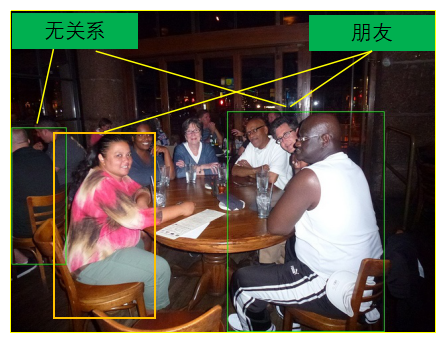
\includegraphics[width=0.58 \textwidth,clip]{images/example-1.png}
                \caption{PIPA-relation数据集\cite{sun2017a}的图例}
        	\label{fig:exp-statistic}
    \end{figure}
    \end{itemize}
\end{frame}

\begin{frame}
    \frametitle{相关工作}
     \begin{block}{社会关系理解模型}
        \begin{itemize}
            \item Dual-glance\cite{li2017dual-glance}利用人周边的物体区域来帮助判断人之间的社会关系
            \item GRM\cite{wang2018deep}通过引入物体类别和关系类别共现频率的先验知识,进而提高预测效果
        \end{itemize}
     \end{block}
     \uncover<3->{
         \begin{block}{模型缺点}
            \begin{itemize}
                \item 场景中的关系往往存在关联,但现有工作忽略人对关系之间的信息交互。
                \item 引入的周边物体特征会把图中所有的关系预测为一样,但存在一张图片包含多种关系类别。
                \item 额外的检测模型检测出物体区域与类别并不一定正确,引入人周边物体的信息存在噪声。
            \end{itemize}
         \end{block}
     }
\end{frame}

\begin{frame}
\frametitle{社会关系图谱}
    \begin{itemize}
       \item 对于图片中的所有人对的社会关系的检测任务,抽象为图片的社会关系图谱生成。
       \begin{figure}
        \centering
            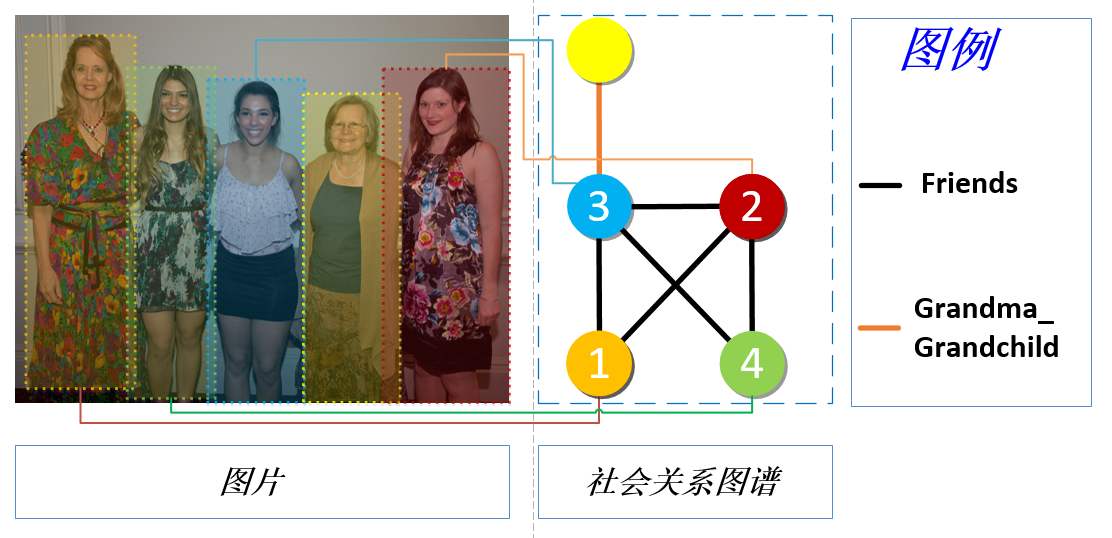
\includegraphics[width=0.70\textwidth]{images/example-3.png}
            \caption{PIPA-relation\cite{sun2017a}数据集中的一个图例}
            \label{fig:example}
        \end{figure}
    \end{itemize}
\end{frame}

\begin{frame}
\frametitle{挑战}
    \begin{block}{挑战}
        \begin{itemize}
            \item 为利用上人对关系间交互的特征,如何设计能捕获人对间社会关系交互的机制。
            \item 如何避免引入不确定的信息,并有效的利用上数据集中已有的标注信息来提升检测效果。
        \end{itemize}
    \end{block}
    \begin{figure}
        \centering
        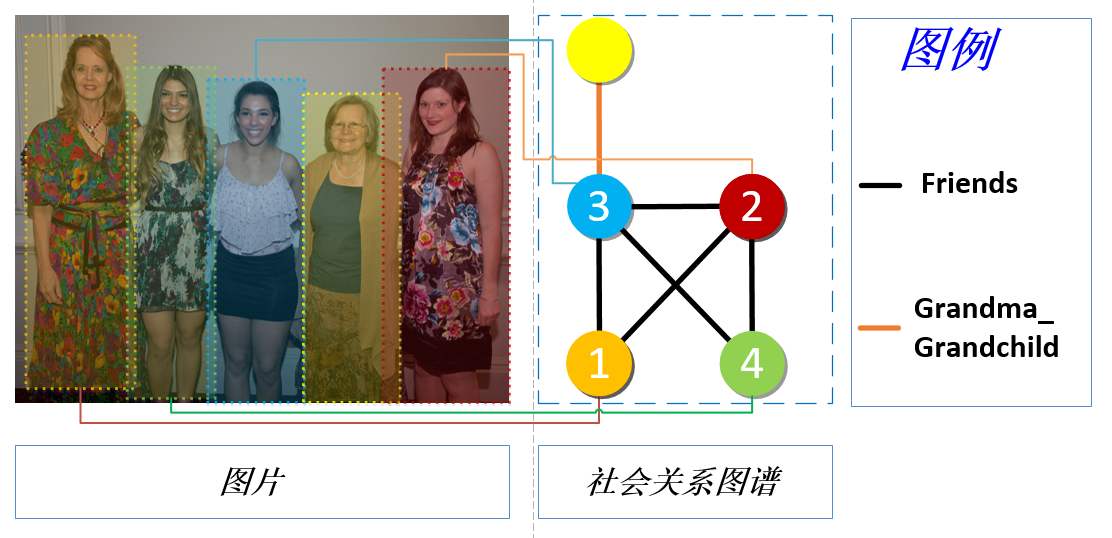
\includegraphics[width=0.48\textwidth]{images/example-3.png}
        \caption{PIPA-relation\cite{sun2017a}数据集中的一个图例}
        \label{fig:example}
    \end{figure}
\end{frame}

\begin{frame}
    \frametitle{本文工作}

            \begin{itemize}
                \item 对于社会关系理解任务,提出了新的概念:{\it 社会关系图谱}
                \vspace*{1.5mm}
                \item 为捕获人对间交互的信息,本文提出了一个迭代的人对关系网络。
                \vspace*{1.5mm}
                \item 提出了一个多任务的损失函数,包括关系损失和关系域损失,并在PISC和PIPA-Relation数据集上验证了PPRN模型的有效性。
                \vspace*{1.5mm}
            \end{itemize}
\end{frame}

\section{PPRN模型}
\begin{frame}
    \frametitle{问题定义}
    \begin{block}{}
        \begin{itemize}
            \item 图片中所有人与人之间的社会关系定义为{\it 社会关系图谱},图的每个节点表示一个人对的关系。
            \item 图谱中关系节点的类别预测可以认为一个图推理问题,并且消息传递是图推理的一种方式。
        \end{itemize}
    \end{block}
    社会关系理解问题可以定义为公式 \ref{eq:model-fram}:
    \begin{equation} \label{eq:model-fram}
        \begin{split}
            x^{*} &= argmax_{x}Pr(x~|~I,B_{i}) \\
            Pr(x~|~I,B_{i}) &= \prod_{i=1}^{N}\prod_{j \neq i}^{N}Pr(x_{i \rightarrow j}^{relation}~|~I,B_{i}) \\
        \end{split}
    \end{equation}
\end{frame}

\begin{frame}
    \frametitle{PPRN模型框架图}
    PPRN包括三个模块: 特征提取模块、消息传递模块、多任务损失模块。
    \begin{figure}
        \centering
        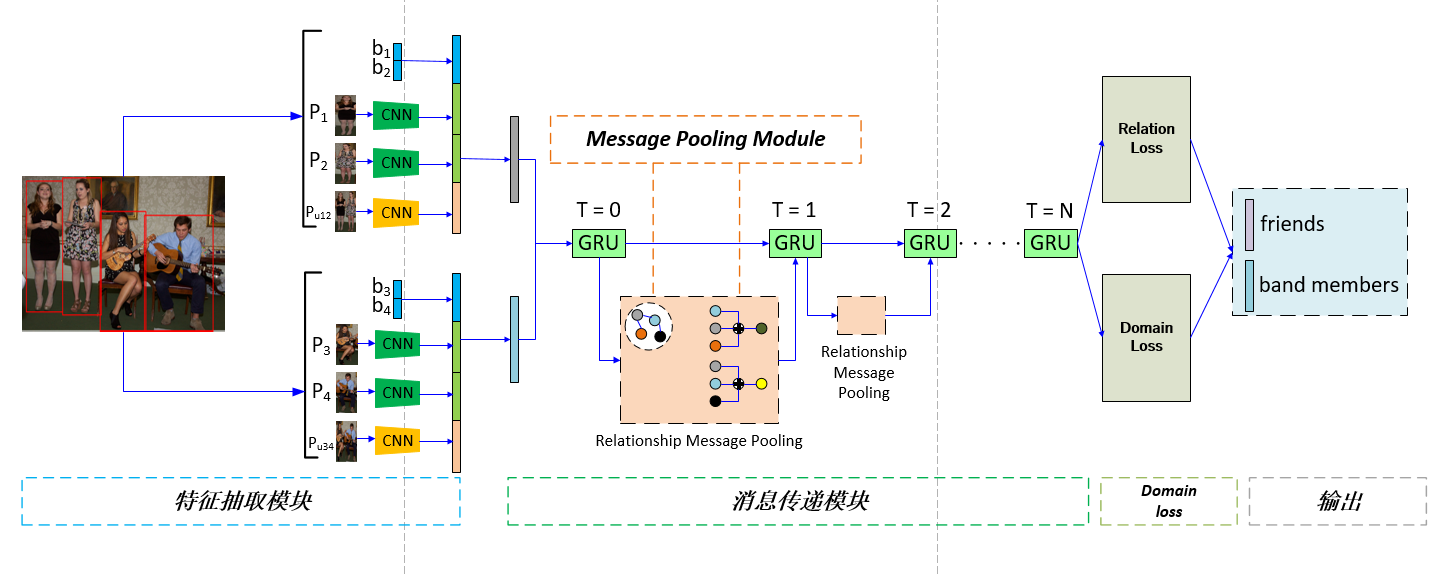
\includegraphics[width=0.98\textwidth]{images/model.png}
        \caption{PPRN的模型框架图}
        \label{fig:PPRN}
    \end{figure}
\end{frame}

%\begin{frame}
%    \frametitle{特征提取模块}
%    \begin{block}{}
%        \begin{itemize}
%            \item 给定一张图片$I$和人的包围盒,对于每个人对首先修剪出三个小块,$p_1,p_2$ 和 $p_{u}$。$p_1$ 和$p_2$是两个个体的区域,$p_u$为两个人区域的联合区域。
%            \item 此外,包围盒的位置信息$b_i^{pos}$同样被使用,$b_i^{pos}$ = $\{ x_{i}^{min},y_{i}^{min}, $ $x_{i}^{max}, ~y_{i}^{max},~ area_{i} \}$ $\in$ $R^5$。
%        \end{itemize}
%    \end{block}
%    \uncover<3->{
%        \begin{block}{}
%                \begin{itemize}
%                    \item $p_1$, $p_2$ 和$p_u$三个区域调整为固定大小输入到三个预训练好的CNNs模型,本文采用的是ResNet-101\footnote{https://download.pytorch.org/models/resnet101-5d3b4d8f.pth},$p_1$和$p_2$共享权重。
%                    \item 人对联合区域特征、单人区域特征和包围盒位置特征通过全连接层得到特征向量$v_h$。
%                \end{itemize}
%        \end{block}
%    }
%\end{frame}

\begin{frame}
    \frametitle{消息传递模块}
     \begin{block}{}
        \begin{itemize}
            \item PPRN采用RNN来解决推理问题,由于GRU的简单和有效,RNNs的神经元采用GRU Unit。
            \item 第t步的隐藏层状态表示当前社会关系图谱的关系节点,每一步GRU的输入来自消息池化模块的输出。
            \item 消息池化模块完成不同人对关系节点的信息传递。
        \end{itemize}
     \end{block}
    % \small{
%    \begin{equation}
%        \label{eq:model-gru}
%        \begin{split}
%        \bm{r}_t &=  \sigma(\bm{W}_{r}[\bm{h}_{t-1}, \bm{x}_t]), \\
%        \bm{z}_t &=  \sigma(\bm{W}_{z}[\bm{h}_{t-1}, \bm{x}_t]), \\
%        \hat{\bm{h}_t} &= tanh(\bm{W}[\bm{r}_t \odot \bm{h}_{t-1}, \bm{x}_{t}])\\
%        \bm{h}_t &= (1 - \bm{z}_t) \odot \bm{h}_{t - 1} + \bm{z}_t \odot \hat{\bm{h}_t} \\
%        \end{split}
%    \end{equation}
%    }
    \begin{figure}
        \centering
        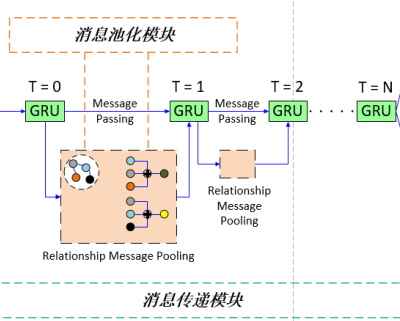
\includegraphics[width=0.38\textwidth]{images/mp.png}
        \caption{消息传递模块}
        \label{fig:PPRN}
    \end{figure}
\end{frame}

\begin{frame}
    \frametitle{消息池化函数}
    \begin{block}{}
        \begin{itemize}
            \item 由于每个GRU会接收多个其它节点的消息,需要一个聚集函数来结合所有的消息得到一个有意义的表征,消息池化函数为每个收到的消息计算一个权重并利用权重来结合这些收到的消息。
            \item 对于在第t步的节点i,其前一步的GRU Unit的隐藏层状态为$h_{i,t-1}$,在第t步来自其他节点的消息表示为$m_{i,t}$,并且$m_{i,t}$为下一步GRU的输入$x_t$。
        \end{itemize}
     \end{block}
     \small{
    \begin{equation}
        \label{eq:model-mp-atten}
    	\bm{m}_{i,t} = ~\sum_{j\neq i} \sigma{(~\bm{w}^T[~\bm{h}_{i,t-1},\bm{h}_{j \to i,t-1}~]) \bm{h}_{j \to i,t-1}}	
    \end{equation}
    }
\end{frame}

%\begin{frame}
%    \frametitle{优化与损失函数}
%    \begin{itemize}
%        \item 给定预测的关系分值$\mathbf{s}^{I,k,rel} \in \mathcal{R}^{|\mathcal{C}|}$和关系域分值$\mathbf{s}^{I,k,dom} \in \mathcal{R}^{|\mathcal{D}|}$,本文采用softmax函数来得到对应的概率分布$p^{I,k,rel} \in \mathcal{R}^{|\mathcal{C}|}$, $p^{I,k,dom} \in \mathcal{R}^{|\mathcal{D}|}$
%        \begin{small}
%        \begin{eqnarray}
%              p_i^{I,k,rel} = \frac{\exp{s_i^{I,k,rel}}}{\sum_{j=1}^{|\mathcal{C}|}{\exp{s_j^{I,k,rel}}}},&
%              i=1,2,\dots,|\mathcal{C}| \label{eq:model-prob-eq} \\
%              p_i^{I,k,dom} = \frac{\exp{s_i^{I,k,dom}}}{\sum_{j=1}^{|\mathcal{D}|}{\exp{s_j^{I,k,dom}}}},&
%              i=1,2,\dots,|\mathcal{D}| \label{eq:model-prob-eq-q}
%        \end{eqnarray}
%        \end{small}
%        \item $\text{N}(I)$返回图片$I$中人对的数量,$\text{L}(\cdot)$是交叉熵损失函数,$\mathcal{I}$是整个图片集。
%        \begin{scriptsize}
%        \begin{equation}
%        \begin{split}
%            \label{eq:model-loss-eq}
%            \mathcal{L} = - \frac{1}{\sum_{I \in \mathcal{I}}\text{N}(I)} \sum_{I \in \mathcal{I}} \sum_{k=1}^{\text{N}(I)} \Big( \sum_{i=1}^{|\mathcal{C}|} \text{L}(y_{i}^{I,k,rel}, p_{i}^{I,k,rel}) + \sum_{i=1}^{|\mathcal{D}|}\text{L}(y_{i}^{I,k,dom}, p_{i}^{I,k,dom}) \Big)
%        \end{split}
%        \end{equation}
%        \end{scriptsize}
%    \end{itemize}
%\end{frame}

\section{实验设计与分析}

\begin{frame}
    \frametitle{数据集}
    %\begin{figure}
%                \centering
%                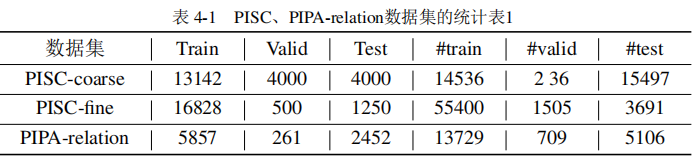
\includegraphics[width=0.68\textwidth]{images/dataset.png}
%                \label{fig:dataset}
%    \end{figure}
    \begin{table}[htpb]
      \centering
      \caption{PISC、PIPA-relation数据集的统计表}
      \label{tab:exp-sta-one}
      \scriptsize
      \scalebox{1.0}{
          \begin{tabular}{c|c|c|c|c|c|c}
            \toprule
            数据集 & Train & Valid & Test & \#train  &  \#valid &  \#test  \\
            \hline
            PISC-coarse & 13142 & 4000 & 4000 & 14536 & 2
            36 & 15497   \\
            \hline
            PISC-fine &  16828 & 500 & 1250 & 55400 & 1505 & 3691 \\
            \hline
            PIPA-relation & 5857 & 261 & 2452 & 13729 & 709 & 5106 \\
            \bottomrule
          \end{tabular}
      }
     \end{table}
    \small
    {
    大多数图片只包含一种关系类型,少数包含2中或多种。}
    \begin{figure}
                \centering
                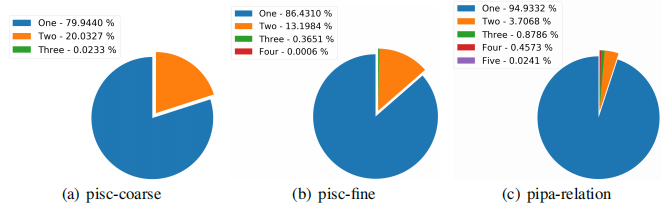
\includegraphics[width=0.58\textwidth]{images/relation-types.png}
                \caption{PISC,PIPA-Relation的关系类别}
                \label{fig:relation-ana}
    \end{figure}
\end{frame}

\begin{frame}
    \frametitle{实验结果}
    \begin{table}[htpb]
      \centering
      \caption{PISC-coarse数据集实验结果,单位为百分比(\%)}
      \label{tab:exp-result-1}
      \scalebox{0.75}{
      \begin{tabular}{c|c|c|c|c}
        \toprule
        模型 & Intimate & Non-Intimate & No Relation & mAP  \\
        \midrule
        Union CNN \cite{lu2016visual} & 72.1 & 81.8 & 19.2 & 58.4   \\
        \midrule
        Pair CNN \cite{li2017dual-glance}  & 70.3 & 80.5 & 38.8 & 65.1   \\
        \midrule
        Pair CNN + BBox + Union \cite{li2017dual-glance}  & 71.1 & 81.2 & 57.9 & 72.2   \\
        \midrule
        Pair CNN + BBox + Global \cite{li2017dual-glance}  & 70.5 & 80.0 & 53.7 & 70.5  \\
        \midrule
        Dual-glance \cite{li2017dual-glance} & 73.1 & \textbf{84.2} & 59.6 & 79.7  \\
        \midrule
        GRM \cite{wang2018deep} & 81.7 & 73.4 & 65.5 & \textbf{82.8}   \\
        \midrule
        PPRN & \textbf{81.9} & 67.3 & \textbf{74.7} & 81.8  \\
        \midrule
      \end{tabular}}
    \end{table}
\end{frame}


\begin{frame}
    \frametitle{实验结果}
    \begin{table}[htpb]
          \centering
          \caption{PISC-fine数据集实验结果,单位为百分比(\%)}
          \label{tab:exp-result-2}
          \scalebox{0.75}{
          \begin{tabular}{c|p{1.5cm}<{\centering}|p{0.8cm}<{\centering}|p{0.8cm}<{\centering}|p{0.8cm}<{\centering}|p{0.8cm}<{\centering}|p{0.8cm}<{\centering}|c}
            \toprule
            模型 & \rotatebox[origin=l]{90}{Friends} & \rotatebox[origin=l]{90}{Family} & \rotatebox[origin=l]{90}{Couple} & \rotatebox[origin=l]{90}{Professional} & \rotatebox[origin=l]{90}{Commercial} & \rotatebox[origin=l]{90}{No Relation} &  \rotatebox[origin=l]{90}{mAP}  \\
            \midrule
            Union CNN  \cite{lu2016visual} & 29.9 & 58.5 & 70.7 & 55.4 & 43.0 & 19.6 & 43.5  \\
            \midrule
            Pair CNN \cite{li2017dual-glance} & 30.2 & 59.1 & 69.4 & 57.5 & 41.9 & 34.2 & 48.2   \\
            \midrule
            Pair CNN + BBox + Union \cite{li2017dual-glance} & 32.5 & 62.1 & 73.9 & 61.4 & 46.0 & 52.1 & 56.9   \\
            \midrule
            Pair CNN + BBox + Global \cite{li2017dual-glance} & 32.2 & 61.7 & 72.6 & 60.8 & 44.3 & 51.0 & 54.6  \\
            \midrule
            Dual-glance\cite{li2017dual-glance} & 35.4 & 68.1 & 76.3 & 70.3 & 57.6 & 60.9 & 63.2  \\
            \midrule
            GRM \cite{wang2018deep} & 59.6 & 64.4 & \textbf{58.6} & 76.6 & 39.5 & 67.7 & 68.7   \\
            \midrule
            PPRN & \textbf{61.0} & 67.1 & 56.2 & \textbf{76.9} & 46.0 & 68.1 & 69.7 \\
            \midrule
            PPRN+d(PPRN+domain loss) & 58.2 & \textbf{68.9} & \textbf{74.6} & 63.3 & \textbf{67.6} & \textbf{70.3} & \textbf{72.0} \\
            \bottomrule
          \end{tabular}
          }
        \end{table}
\end{frame}

\begin{frame}
    \frametitle{PIPA-relation实验结果与分析}
        %\begin{figure}
%                \centering
%                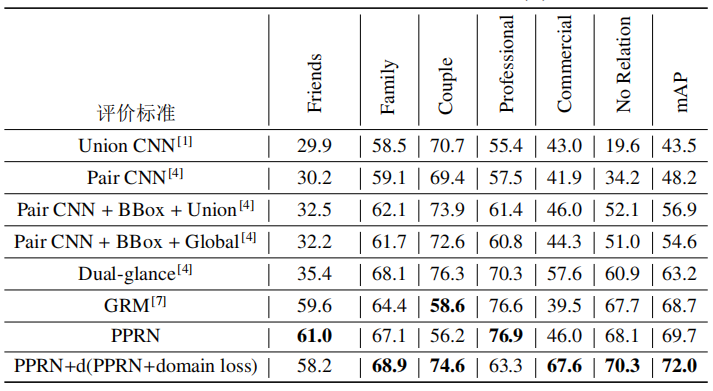
\includegraphics[width=0.45\textwidth]{images/pisc-fine.png}
%                \caption{\tiny{PISC-fine实验结果}}
%                \label{fig:pisc-fine}
%         \end{figure}
         %\begin{figure}
%                \centering
%                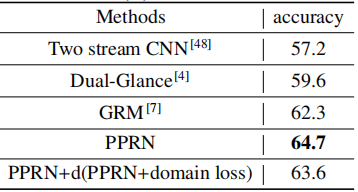
\includegraphics[width=0.30\textwidth]{images/pipa.png}
%                \caption{\tiny{PIPA-relation实验结果}}
%                \label{fig:pisc-fine}
%         \end{figure}
        \begin{table}[htpb]
          \centering
          \caption{PIPA-relation实验结果,单位为百分比 (\%) }
          \label{tab:exp-pipa-table}
          \scalebox{0.68}{
          \begin{tabular}{c|c}
            \toprule
            模型 & accuracy \\
            \midrule
            Two stream CNN \cite{zhang2015beyond} & 57.2 \\
            \midrule
            Dual-Glance \cite{li2017dual-glance} & 59.6 \\
            \midrule
            GRM \cite{wang2018deep} & 62.3 \\
            \midrule
            PPRN & \textbf{64.7} \\
            \midrule
            PPRN+d(PPRN+domain loss)  & 63.6 \\
            \bottomrule
          \end{tabular}
          }
        \end{table}
        \begin{block}{结论与分析}
            \begin{itemize}
                 \item PPRN在fine-level的识别任务上超过了之前所有的模型,但是在coarse-level轻微的低于之前最优模型。
                 \item 通过引入关系域损失,模型在PISC-fine数据集上有显著的提高。模型通过同时优化关系损失和关系域损失,两个任务的特征共享并且两个任务的相互约束能帮助区分属于不同关系域的关系。
            \end{itemize}
        \end{block}

\end{frame}

\begin{frame}
    \frametitle{实验结果分析}

     \begin{table}[htb]
        	\vspace*{-3.5pt}
        	\centering
        	\caption{不同池化策略和引入周边物体区域的实验结果}
            \label{tab:exp-mp-variant}
        	\vspace*{-0.5mm}
            \scalebox{0.58}{
        	\begin{tabular}{c|c|c|c|c}
        		\toprule
        		\multirow{2}{*}{模型} &
        		\multicolumn{2}{c|}{PISC coarse} &
        		\multicolumn{2}{|c}{PISC fine}  \\
        				 & accuracy & mAP & accuracy & mAP  \\
        		\midrule
        		RCNN & - & 63.5 & - & 48.4 \\
        		\midrule
        		PPRN(max pooling) & 74.3 & 80.8 & 64.1 & 68.1 \\
        		\midrule
        		PPRN(avg pooling) & 74.6 & 80.1 & 63.8 & 68.3 \\
        		\midrule
        		PPRN(attention) & \textbf{75.1} & \textbf{81.8} & \textbf{65.7} & \textbf{69.7} \\
        		\midrule
        		PPRN+d  & - & - & \textbf{66.2} & \textbf{72.0} \\
                \midrule
        		PPRN+d+obj  & 74.9 & 81.2 & 65.3 & 69.1 \\
        		\midrule
    	       \end{tabular}
            }
    \end{table}
    \begin{block}{结论与分析}
            \begin{itemize}
                 \item RCNN,Dual-glance和GRM模型均引入额外的Faster-RCNN模型来提取图片人周围的问题特征,但是在PPRN中引入后效果反而出现轻微下降。
                 \item 人对关系交互的特征已经覆盖了人周边物体区域的特征。
            \end{itemize}
        \end{block}

\end{frame}

\begin{frame}
    \frametitle{样例分析}
          \begin{figure}
                \centering
                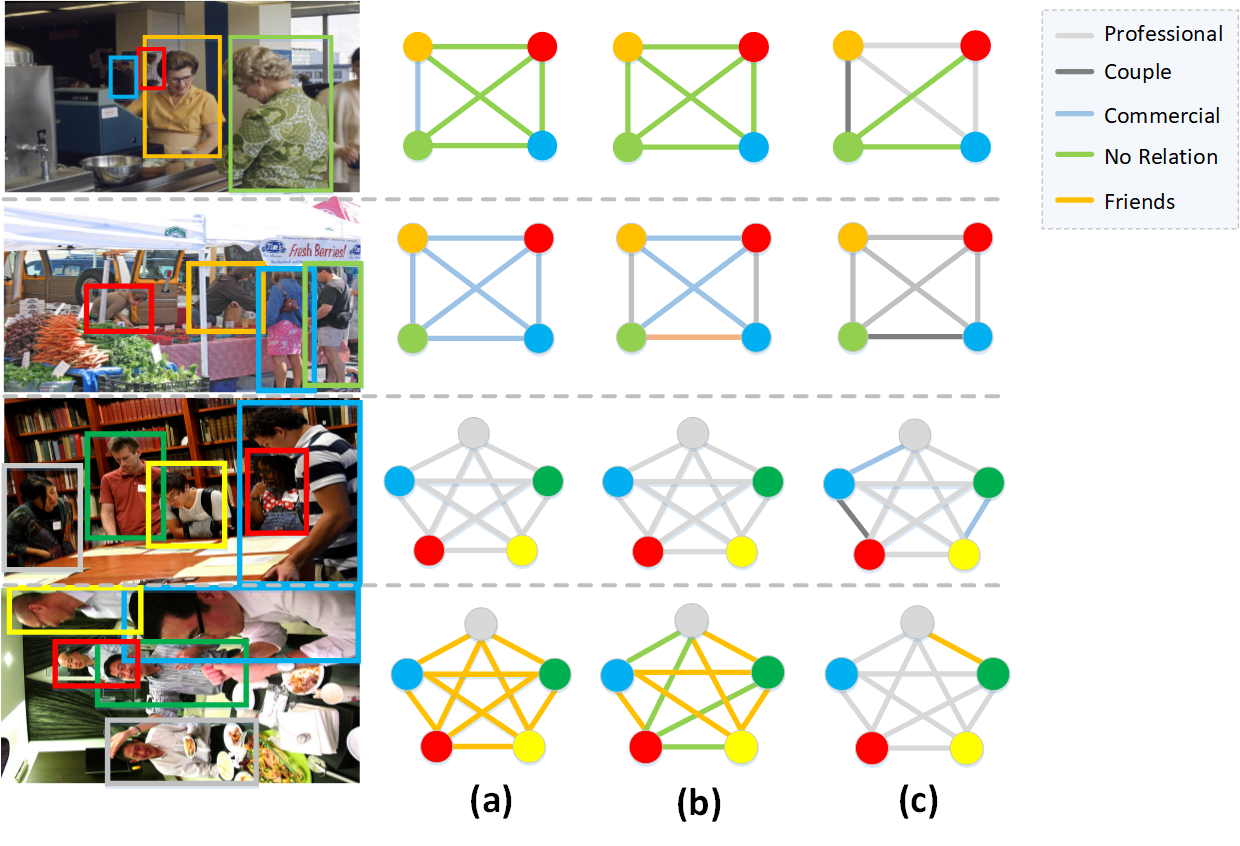
\includegraphics[width=0.7\textwidth]{images/case_study.png}
                \caption{(a)标注 (b) PPRN  (c) GRM }
                \label{fig:pisc-fine}
         \end{figure}
\end{frame}

\section{总结与展望}

\begin{frame}
    \frametitle{总结与展望}
    \begin{block}{总结}
         \begin{itemize}
         \item 提出一个生成图片社会关系图谱的人对关系网络,PPRN利用RNNs在一个在不同人对间进行推理,在特征提取的基础上进一步提升了识别的效果。
         \item 提出引入关系域损失,提升关系识别的效果
         \item 在现有的大型社会关系理解数据集验证了PPRN模型的有效性。
         \end{itemize}
    \end{block}
    \begin{block}{展望}
        \begin{itemize}
            \item 引入更多的未标注人的标签信息,例如人的年龄和性别。
            \item 将当前方法应用到视频理解的任务上,例如视频的人物关系检测。
        \end{itemize}
    \end{block}
\end{frame}

\section{附录}

\begin{frame}
    \frametitle{攻读硕士学位期间科研成果}
    \small{
         \begin{enumerate}
         \item 中山大学.一种基于二次主题空间投影的场景图谱低维空间嵌入方法; (专利,学生第一作者,申请未公开)(与本文第1章关于场景图谱的内容相关)
         \item Understanding Social Relationship with Person-pair Relations. 投稿于IJCAI-2019(CCF-A类会议,学生第一作者,录用边缘)(与本文第3、4章相关)
         \end{enumerate}
    }
\end{frame}

\begin{frame}
    \frametitle{盲审意见修改}
    \small{
         \begin{enumerate}

         \item 此外,文章的图是否部分引用了现有文献的?这个需要作者检查,如果用了别人的图,需要加标注\\
         {\kai 论文17页,图2-5,已添加参考文献原图的引用。
                论文38页,图4-1,已添加参考文献原图的引用}
         \item 在进行与已有工作对比时,除了展示本文方法的优势之外,建议也分析一下
                    所存在的劣势\\
         {\kai 论文45页,实验分析的第五点添加了关于本方法的一些劣势,例如在粗粒度的任务上未取得最优的效果}
         \item 绪论,实验设计等章节部分内容表述不明确,需要仔细检查,修改 \\
         {\kai 已修改论文绪论、实验部分表述}
         \end{enumerate}
    }
\end{frame}

\begin{frame}
    \frametitle{初审意见修改}
    \small{
         \begin{enumerate}

         \item 答辩ppt英文题目与论文题目不一致\\
         {\kai 已修正}
         \end{enumerate}
    }
\end{frame}

\begin{frame}
    \centerline{\large{感谢各位评审老师的聆听与指导!}}
\end{frame}

\subsection{ }
\begin{frame}[allowframebreaks]
    \frametitle{参考文献}
    \tiny
    %\bibliographystyle{plain}
    %\bibliographystyle{TJUThesis}        % bst文件名,注意不要后缀
    \printbibliography
    %\bibliography{reference}
\end{frame}

\end{document}
